

\section{Pushing an evasive esoteric streamway and plumbing the depths of humour}

\margininbox{Esoterica}{
		\begin{itemize}
		\item James O'Hanlon
		\item William French
		\end{itemize}
}{\explo}

\paragraph{Preamble}
After a leasurely shit, me and James are off to check out \passage{Esoterica} and maybe discover why a lead so close to camp has been ignored for 4 years.
\name{William French}
\paragraph{The push} I have descended where no man has descended before. Pushing for the first time was very thrilling even if 98$\%$ of the work was done by William. 
Setting off at 12.00\,am we went to find \passage{Esoterica}. I was doubtful we would find it as Tetley had tried 3 times and failed, however we went with high hopes.
After a TWATTY descent through \passage{Cheetah} we ventured \passage{Prince Consort Road} and came to a suspicious looking pitch. It was \textit{pictouresk?}...  a pretty pitch with a pool directly above another.

We used rope that was already available and bolted to descend down to the bottom pool but alas nothing. After I quickly checked that top pool for a lead we moved on. William then found a piece of paper with PSS 12. Success! This is the clue that we were looking for. The other piece of paper was covered in mud and after pouring water on it, it revealed the message.  \textit{`Push the rift downstream'}. This felt like a treasure hunt and we were hot under the trail.

\begin{marginfigure}
\centering
  \frame{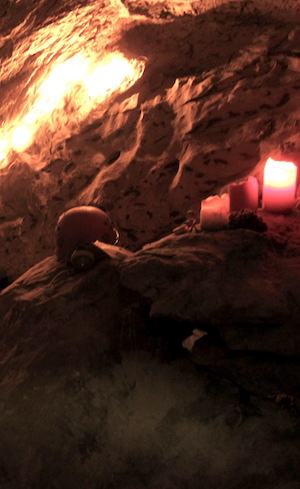
\includegraphics[width=\linewidth]{images/2014/james-yourmum-2014/life_at_xray.jpg}}
  \caption{The `fairy lights' of camp \protect\passage{X-Ray} emit a reassuring glow through the night \pic{Jarvist Frost}}
\end{marginfigure}

After a brief crawl we found  \passage{Esoterica} and we began to go through the rift. After some twat we reached the end of the last push and reached a pitch that had not been rigged. Excited I waited for William to bolt… and waited … and waited. After what felt like an age William had finished and allowed me to go down first. Suddenly the bitter cold had vanished and as my feet hit the bottom of the pitch I was elated!! William named the pitch `\passage{Your Mum}'. A rather ingenious name eg. The pitch `\passage{Your Mum}' was wet. After surveying the pitch we headed back rather exhausted. 

Reflecting over these two weeks at Expo I feel like I've achieved a lot. Let's hope next year will be just as good.
\name{James O'Hanlon}

\paragraph{Epilogue}  It's pretty tight and wet which may explain why no one has really been there. There is also a dry climb right off the start which may be a going lead. 
\name{William French}

%\begin{figure*}[h!]
 %     \checkoddpage \ifoddpage \forcerectofloat \else \forceversofloat \fi
 %     \centering
 %             \frame{\includegraphics[width=\linewidth]{"images/2014/james-yourmum-2014/tent-on-surface".jpg}} 
 %      \label{tent at dusk}
 % \caption{As the sun sets, the cavers retreat to their tents. --- Rhys Tyers}
%\end{figure*}
